\documentclass[10pt, letterpaper]{article}
\usepackage[letterpaper, top=2.2cm, bottom=2.4cm, left=2.3cm, right=2.3cm]{geometry}
\usepackage[T1]{fontenc}
\usepackage{amsmath, amssymb}
\usepackage{newtxtext}
\usepackage[scaled=0.92]{helvet}
\let\Bbbk\relax
\usepackage{newtxmath}
\usepackage{graphicx}
\usepackage{booktabs}
\usepackage{titlesec}
\usepackage{xcolor}
\usepackage{caption}
\usepackage{fancyhdr}
\usepackage[hidelinks]{hyperref}

\definecolor{sec}{RGB}{22,45,74}
\titleformat{\section}{\sffamily\large\bfseries\color{sec}}{\thesection}{0.6em}{}
\captionsetup{labelfont={bf,sf}, font=small, labelsep=period}
\renewcommand{\thefigure}{S\arabic{figure}}
\renewcommand{\thetable}{S\arabic{table}}
\pagestyle{fancy}\fancyhf{}
\renewcommand{\headrulewidth}{0pt}
\fancyhead[L]{\sffamily\footnotesize\color{sec}Supplementary Information}
\fancyfoot[C]{\sffamily\footnotesize S\thepage}

\title{\sffamily\bfseries\color{sec}Supplementary Information\\[2pt]
\large\mdseries Place-field repetition is what a predictive map must do when self-motion cannot
resolve it: a cognitive map represents space only up to the symmetries self-motion cannot break}
\author{\sffamily Manas Venkata Sai Ravulapalli}
\date{}

\begin{document}
\maketitle

\noindent This document collects supporting figures for the main text. All panels are generated
directly from the result files by \texttt{project5\_symmetry/analysis/make\_paper\_figures.py} and
\texttt{rate\_maps.py}; no values are entered by hand.

\section{Place-field rate maps, all extracted units}

The main-text place-cell figure shows a small number of example units per condition. To show that
this selection is representative rather than chosen, the following figures give the full set of
extracted units for each condition, ranked by Skaggs spatial information and left otherwise
unselected. Each tile is one unit's mean firing-rate map over the arena, smoothed for display and
normalised to its own peak.

\begin{figure}[h!]
\centering

\includegraphics[width=\textwidth]{figures/figS_units_s1_full.pdf}
\caption{Asymmetric arena, full head-direction encoding. Units carry single, sharp place fields.}
\end{figure}

\begin{figure}[h!]
\centering

\includegraphics[width=\textwidth]{figures/figS_units_s2_full.pdf}
\caption{$C_2$ arena, full head-direction encoding. With the full compass available the fields do
not systematically repeat.}
\end{figure}

\begin{figure}[h!]
\centering

\includegraphics[width=\textwidth]{figures/figS_units_s2_axis.pdf}
\caption{$C_2$ arena, \textit{axis} encoding. The encoding is invariant under the $180^\circ$
rotation, and fields repeat at $180^\circ$-related locations across the population.}
\end{figure}

\begin{figure}[h!]
\centering

\includegraphics[width=\textwidth]{figures/figS_units_s4_const.pdf}
\caption{$C_4$ arena, \textit{const} encoding. The encoding is invariant under the full $C_4$
group, and fields repeat at all four $90^\circ$-related locations.}
\end{figure}

\clearpage
\section{Cell-type composition}

\begin{figure}[h!]
\centering

\includegraphics[width=0.85\textwidth]{figures/figS_celltypes.pdf}
\caption{The trained population is a realistic cell-type mixture, scored by the criteria applied
to real recordings. (\textbf{a}) Fraction of units classified as place cells (Skaggs spatial
information above threshold) and as border-modulated (a third or more of the rate-map mass in the
outer ring), by head-direction encoding, pooled across arenas. The composition is stable across
encodings. (\textbf{b}) Fields per place cell by encoding and arena ($C_1/C_2/C_4$): it rises with
both encoding invariance and arena symmetry, from $1.78$ to $3.39$, the multi-field signature of
the fold. Folding rearranges where fields sit and multiplies them without changing the cell-type
makeup. Bars are mean $\pm$ s.e.m.\ over networks.}
\end{figure}

\clearpage
\section{Population manifolds of the topology arenas}

\begin{figure}[h!]
\centering

\includegraphics[width=\textwidth]{figures/fig4_geometry.pdf}
\caption{Position-conditioned population manifolds for the four topology arenas, PCA to three
dimensions (one point per passable cell, coloured by angle around the arena centre). Position is
mapped smoothly in every arena, but the manifolds are high-dimensional: three principal
components capture only $34$--$41\%$ of the variance, and no low-dimensional loop is visible even
for the annulus ($b_1 = 1$) or the theta and figure-8 arenas ($b_1 = 2$). This is consistent
with the persistent-homology analysis, which does not recover the arenas' loop topology (main
text, Limitations): the code is metrically organised well before, and without ever cleanly
acquiring, the arena's topology.}
\end{figure}

\clearpage
\section{Diffusion-map geometry of the manifolds}

Diffusion maps embed a point cloud through the eigenfunctions of a Markov random walk built on it,
so the embedding respects diffusion distance --- a density-robust, geometry-aware metric --- and
the eigenvalue spectrum reads out intrinsic dimension. Both structures survive this nonlinear
readout.

\begin{figure}[h!]
\centering
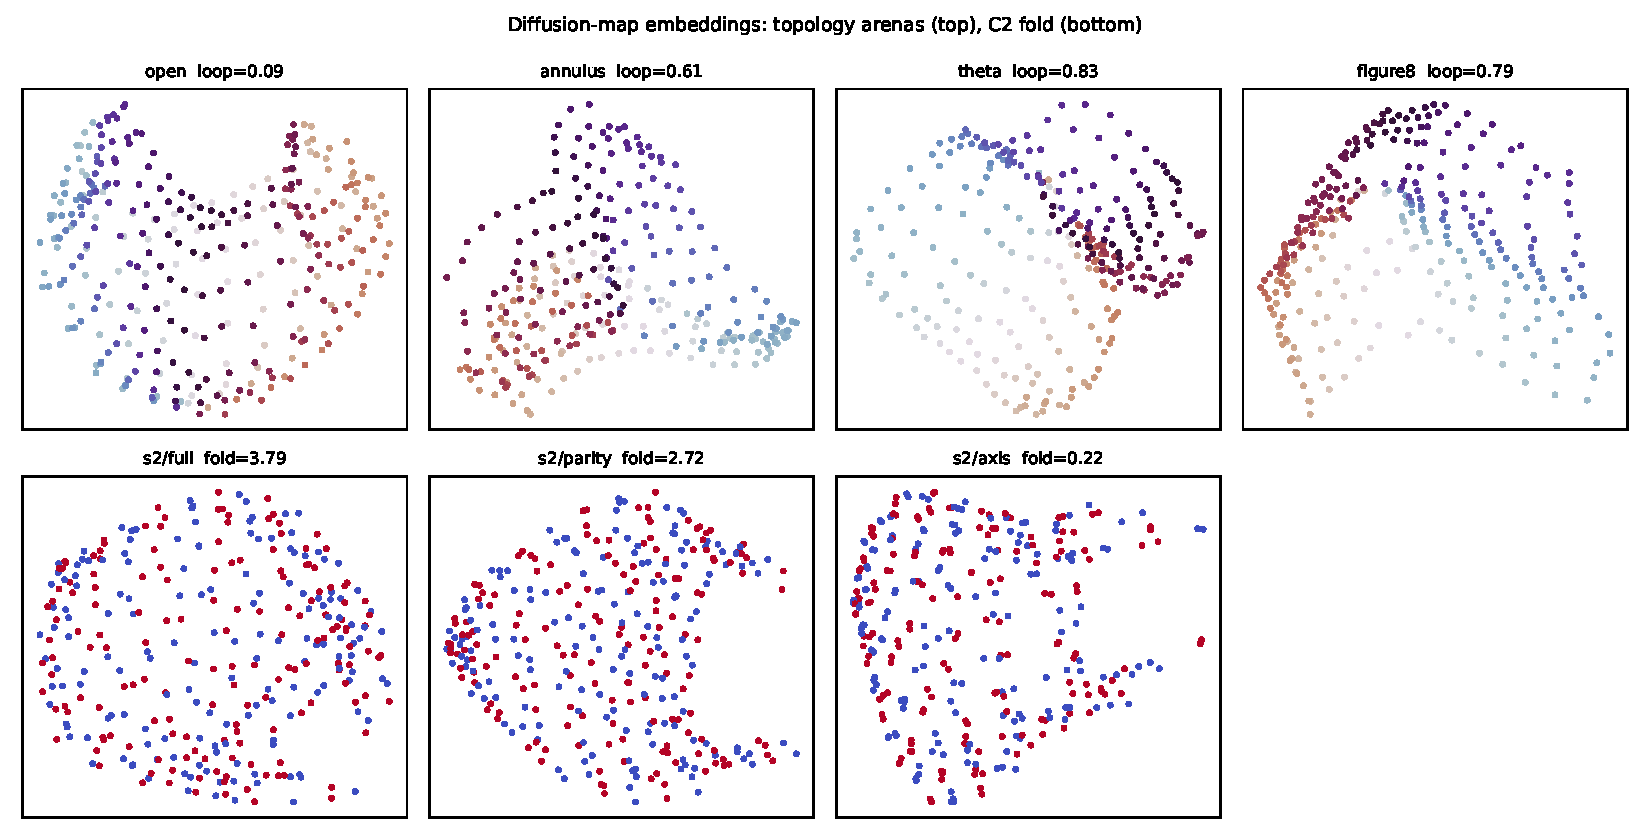
\includegraphics[width=\textwidth]{figures/figS_diffusion.pdf}
\caption{Diffusion-map embeddings. \textbf{Top:} topology arenas, coloured by arena angle. The
open arena shows no angular loop in the leading diffusion coordinates (loop score $0.09$), whereas
the annulus, theta and figure-8 arenas do ($0.61$--$0.83$); the manifolds nonetheless remain
moderately high-dimensional (intrinsic dimension $5$--$7$), consistent with the persistent-homology
result that a single loop is recoverable but higher-genus topology is not. \textbf{Bottom:} the
$C_2$ fold, coloured by orbit tag. The diffusion distance between a position and its $180^\circ$
image, in units of the distance to a spatial neighbour, is $3.79$ under \textit{full} and $2.72$
under \textit{parity} but collapses to $0.22$ under \textit{axis}: the fold is a property of the
diffusion geometry, not of any linear projection.}
\end{figure}

\clearpage
\section{The wake manifold has the topology of $X/G$, not $X$}

The previous section's diffusion-distance collapse (position vs.\ $180^\circ$ image, $0.22$ under
\textit{axis} against $2.72$--$3.79$ for the non-invariant encodings) says the fold shows up in a
nonlinear, density-robust metric and is not an artefact of a linear projection. It does not by
itself say what shape the manifold has taken. We ask that question directly: is the population
code, once folded, a map of the physical arena $X$, or of the quotient $X/G$?

If it is $X/G$, a position and its $180^\circ$ image under \textit{axis} should not merely be
\emph{closer} than average in neural space, they should be nearly the same point, to within the
noise the network's own stochasticity sets, while \textit{full} networks (nothing to fold onto)
keep them as far apart as any unrelated pair. We tested this on the $C_2$ arena, across five
independently trained networks per encoding: the ratio of neural distance between a position and
its $180^\circ$ image to the neural distance between a random pair of positions.

\begin{figure}[h!]
\centering
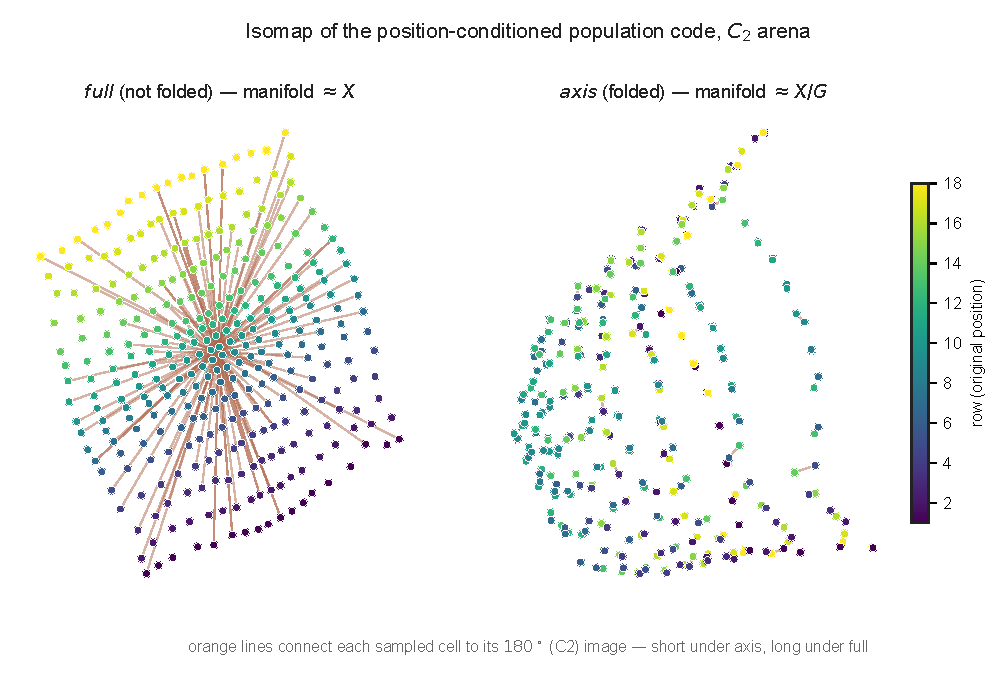
\includegraphics[width=0.9\textwidth]{figures/figS_fundamental_domain.pdf}
\caption{Isomap embedding (geodesic, 2 nearest-neighbour graph, 2 components) of the
position-conditioned population code in the $C_2$ arena, coloured by original row. Lines connect a
sample of cells to their $180^\circ$ image. Under \textit{full} (left) the embedding recovers the
arena's own layout and partner lines span the full manifold. Under \textit{axis} (right) partner
lines collapse to near zero length: the two symmetry-related halves of the arena have been written
onto (approximately) the same manifold, the glued fundamental domain the Theorem predicts, not the
unfolded square.}
\label{figS:funddomain}
\end{figure}

Table~\ref{tabS:funddomain} gives the ratio for each of the five seeds per encoding. Under
\textit{axis} a position sits, on average, $0.17$--$0.18$ of a random pair's distance from its own
$180^\circ$ image; under \textit{full} the same ratio is $0.85$--$0.89$, statistically
indistinguishable from a pair with no relationship at all. The separation is complete across all
five seeds of each encoding (Mann--Whitney $U=0$, $p=0.004$, the exact floor at $n=5$ vs.\ $5$).
This is the topological reading of the quotient law: the network does not merely fail to
discriminate $180^\circ$-related positions, as the orbit-phase decoding in the main text already
shows; it collapses them onto (approximately) the same point of a folded manifold, so that the
wake code under a fully $G$-invariant compass is a map of the fundamental domain, glued, not a map
of the arena with two indistinguishable regions on it.

\begin{table}[h!]
\centering
\caption{Ratio of neural distance between a position and its $180^\circ$ image to the neural
distance between a random pair of positions, $C_2$ arena, five independently trained networks per
encoding.}
\label{tabS:funddomain}
\begin{tabular}{lccccc}
\toprule
encoding & seed 0 & seed 1 & seed 2 & seed 3 & seed 4 \\
\midrule
\textit{axis} & $0.172$ & $0.179$ & $0.179$ & $0.167$ & $0.170$ \\
\textit{full} & $0.877$ & $0.851$ & $0.869$ & $0.889$ & $0.884$ \\
\bottomrule
\end{tabular}
\end{table}

\paragraph{Methods.} \texttt{analysis/fundamental\_domain\_isomap.py}. For each of five seeds per
encoding, hidden states were collected from the network's own trajectories (20{,}000 states,
matching the orbit-phase decoding protocol) and averaged per arena cell to give a
position-conditioned population code (324 cells). The $180^\circ$ partner of each cell is
$(19-\text{col}, 19-\text{row})$; the random-pair baseline pairs each cell with an independently
shuffled cell, seeded per network. The Isomap embedding (Fig.~\ref{figS:funddomain}) uses one
representative network per encoding, 8 nearest neighbours, 2 components; the ratio statistics
(Table~\ref{tabS:funddomain}) use the raw 500-dimensional hidden state, not the 2-D embedding, so
the effect is not a projection artefact. Values in \texttt{Report/data/fundamental\_domain\_isomap.csv}.

\clearpage
\section{Initialization and learning speed}

The recurrent matrix is not initialized at random alone: the architecture adds a
leaky-integrator term $(1 - 1/\tau)\,I$, and a comment in the original code records that a
Kaiming initialization was tried and discarded because it ``blows up''. We varied the
initialization along three axes --- the identity time constant $\tau$, the gain of the random
component, and its structure --- and summarised each run by the area under its training-loss
curve (Fig.~\ref{figS:init}). Learning speed ordered monotonically with the amount of random
recurrent mixing present at initialization. A pure leak, $W = 0.5\,I$ with no random recurrence,
learned fastest; larger random components learned more slowly, and the two Kaiming variants were
slowest of all. Neither Kaiming variant diverged: its loss fell monotonically to within $33\%$
of the default by area, with no sign of instability. The blow-up recorded in the original comment
belongs to the plain recurrent cell, not to the layer-normalised cell this network uses. This
analysis bears on training dynamics rather than on the symmetry results of the main text, and is
reported here for completeness.

\begin{figure}[h!]
\centering

\includegraphics[width=0.75\textwidth]{figures/figS_init.pdf}
\caption{Learning speed by recurrent initialization, measured as area under the training-loss
curve (lower is faster), ranked. A pure leak with no random recurrence learns fastest; adding
random mixing slows learning monotonically. The abandoned Kaiming initialization is slowest but
converges without instability. Dots are individual networks.}
\label{figS:init}
\end{figure}

\clearpage
\section{CA1 reanalysis: exploratory and non-diagnostic}

The main text (Fig.~6b) reports a predictive network's own prediction for a city-block
maze: same-orientation alleys are translation-related (the compass reads the same) and orthogonal
alleys are rotation-related, so a repeating cell's fields should share a directional preference
across same-orientation alleys and not across orthogonal ones. Here we ask whether that signature,
confirmed in the model, is visible in real neurons.

We reanalysed the CA1 recordings of Hockeimer et al.\ (2023), in which rats foraged a city-block maze
whose alleys run in two orthogonal orientations. Within a repeating cell, the directional index of
same-orientation field pairs is positively correlated ($r = 0.23$; $127$ pairs, $40$ cells, $5$
rats; Fig.~\ref{figS:ca1}), and pairs in orthogonally-oriented alleys are uncorrelated ($r =
-0.06$).

This dataset cannot, however, separate the fold from a conjunctive place-by-direction code, which
would produce the same correlation without any folding: a cell with a global directional
preference has consistently signed directional indices across all its same-orientation fields. Two
controls make the ambiguity explicit. The correlation is if anything stronger among
\emph{non-repeating} cells ($r = 0.63$, though only $12$ pairs), so it does not require the field
repetition the fold predicts; and the directional index is a stable per-cell property
(mixed-effects intraclass correlation $0.31$), so a cell-scramble that preserves each cell's
overall directionality reproduces the correlation ($r = 0.52$, above the observed value). We
therefore report the CA1 correlation as \emph{consistent with} the quotient but not diagnostic of
it; separating the two accounts requires per-cell head-direction tuning, or the
parallel-versus-radial manipulation of Grieves et al.\ (2016) read out directionally.

\begin{figure}[h!]
\centering
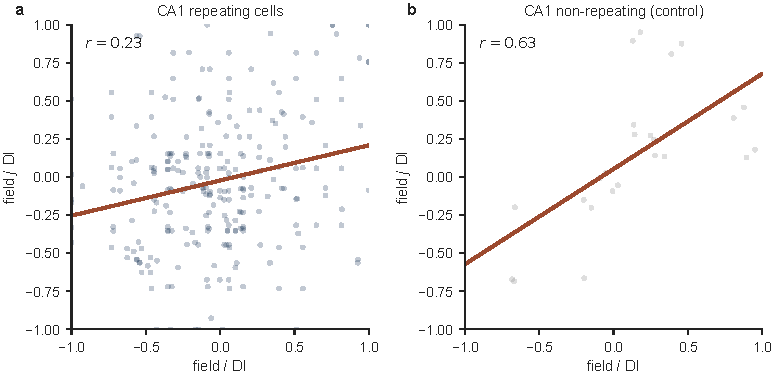
\includegraphics[width=0.72\textwidth]{figures/figS_ca1.pdf}
\caption{Exploratory reanalysis of CA1 city-block data (Hockeimer et al.\ 2023): consistent
with the quotient but not diagnostic. (\textbf{a}) For repeating cells, same-orientation field-DI
pairs are weakly positively correlated ($r=0.23$). (\textbf{b}) Non-repeating cells show a similar
correlation ($r=0.63$), so the effect does not require the repetition the fold predicts, and a
directionality-matched cell-scramble reproduces it ($r=0.52$). The correlation is therefore not
separable from a conjunctive place-by-direction code; a decisive test needs per-cell
head-direction tuning.}
\label{figS:ca1}
\end{figure}

\clearpage
\section{Coset versus phase: folded, not broken}

Figure~\ref{figS:cosetphase} plots within-domain position ($R^2_{\text{domain}}$) against
orbit-phase accuracy for every network and encoding in the main sweep. The two quantities move
independently: domain position is high (typically $0.8$--$0.9$) regardless of whether the
encoding is invariant, while phase accuracy is high only for the non-invariant encodings and sits
at the null for the invariant ones in a symmetric arena. This is the pattern a fold, rather than a
collapse of the spatial code altogether, predicts: the network keeps a reproducible map of the
fundamental domain and loses only which copy of it produced the current state.

\begin{figure}[h!]
\centering
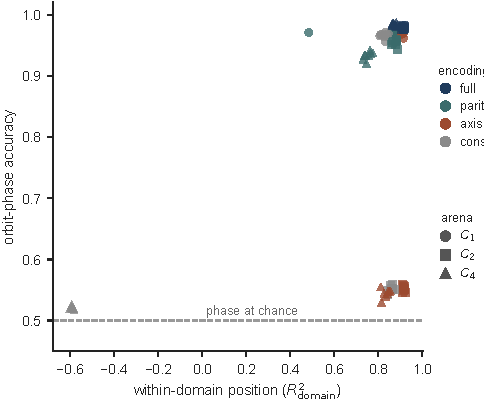
\includegraphics[width=0.72\textwidth]{figures/figS_coset_phase.pdf}
\caption{Within-domain position ($R^2_{\text{domain}}$) versus orbit-phase accuracy, every
network and encoding, arenas $C_1$/$C_2$/$C_4$. High domain $R^2$ co-occurs with high phase
accuracy for the non-invariant encodings (\textit{full}, \textit{parity}) and with chance-level
phase accuracy for the invariant ones (\textit{axis}, \textit{const}) in a symmetric arena: the
coset is preserved while the phase is not. The point near $R^2_{\text{domain}} = -0.6$ is
\textit{const} in the $C_4$ arena, folded by the full $C_4$ group in a way a $C_2$-based readout
cannot see (main text).}
\label{figS:cosetphase}
\end{figure}

\section{The fold as a manifold, not just a decoder score: compartment maze}

Every fold reported in the main text is a classifier's cross-validated accuracy. Figure~\ref{figS:isomap}
asks the same question with no decoder at all: does the shape of the population activity itself
look like one room or two? We took the horizon-sweep networks (main text) at $k=3$ and built an
Isomap embedding of the wake population state (cosine metric, 150 nearest neighbours, following
Levenstein et al.\ (2024)), coloured by which physical room produced each state --- a label
the embedding never sees. For each of the 36 matched positions in the two rooms we measured the
distance, in the embedding, between room A's and room B's centroid for that position, normalised
by the embedding's overall spread. Under translation, where the Theorem predicts folding, this
matched-cell distance is $0.13 \pm 0.01$ (mean $\pm$ s.d., $n=8$ seeds): room B's copy of a
position embeds almost exactly where room A's does. Under rotation, where the compass turns with
the room and the Theorem does not predict folding, the same distance is $1.31 \pm 0.16$, an order
of magnitude larger (exact two-sided Mann--Whitney $U$, $n=8$ vs.\ $8$, $p=1.55\times10^{-4}$,
the floor for this $n$). The result is unchanged embedding into three dimensions instead of two
($0.17 \pm 0.02$ vs.\ $1.72 \pm 0.22$, same $p$), so the two-dimensional panel below is not
compressing structure that only separates in higher dimensions.

The same check at the other completed horizon-sweep values (main text) shows this geometric
fold is itself prediction-dependent, independently of any decoder: at $k=0$, the autoencoder
control with no rollout to predict, translation and rotation are geometrically
indistinguishable ($0.20 \pm 0.01$ vs.\ $0.21 \pm 0.03$, $p=0.23$, not significant). At $k=1$
the two are already well separated ($0.19 \pm 0.01$ vs.\ $0.26 \pm 0.04$,
$p=1.55\times10^{-4}$), and the separation grows substantially larger by $k=3$ above. This
mirrors the main text's decoder-based finding that folding requires a predictive objective, now
shown directly in the shape of the population code rather than in a classifier's score.

\begin{figure}[h!]
\centering
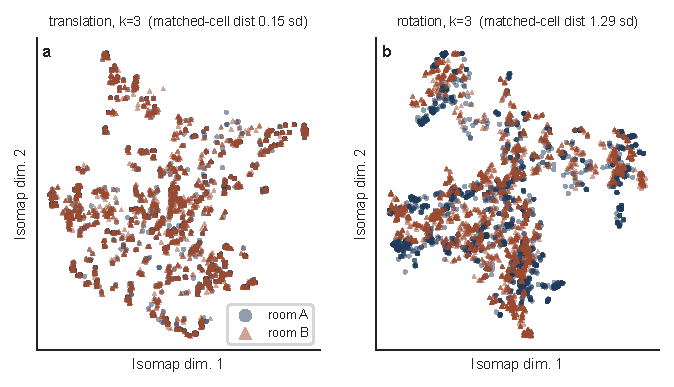
\includegraphics[width=0.95\textwidth]{figures/figS_isomap_compartment.pdf}
\caption{Isomap embedding of the wake population state, compartment maze, $k=3$, one
representative network per condition (the matched-cell-distance statistic in the text is over
all 8 seeds). Each point is one moment in time; colour is the room the agent actually occupied
(never shown to Isomap). \textbf{(a)} Translation: rooms A and B are thoroughly interleaved --
the network's internal state cannot tell them apart. \textbf{(b)} Rotation: the two rooms occupy
visibly more separated regions of the embedding.}
\label{figS:isomap}
\end{figure}

\clearpage
\section{Nonlinear decoders confirm the chance-level fold}

The main text reports orbit phase from a linear (logistic) decoder, so a natural worry is that the
folded encodings carry orbit-phase information a linear readout cannot reach. They do not. On the same
$C_2$ population states, a $k$-nearest-neighbour decoder and a multi-layer perceptron also sit at chance
for the invariant encodings (\textit{axis}: $0.537$ and $0.535$; \textit{const}: $0.531$ and $0.531$;
$n=6$), and both recover orbit phase for the non-invariant encodings (\textit{full} and \textit{parity},
every network $\ge 0.90$). The orbit-phase information is absent from the folded code, not merely hidden
from a linear readout.

\section{Three single-cell readouts fail in the same way}

An invariant compass makes the code look symmetric whether or not the arena is, so single-cell measures
of symmetry report a fold even in the $C_1$ arena, where none can exist. Three readouts we tried early
have exactly this defect, which is why the main text reports orbit-phase decoding --- whose null
survives the $C_1$ arena --- as primary throughout.

\emph{Rotational autocorrelation} is $\mathrm{RA} = P_0 - P_2$ in the isotypic power spectrum
(Fig.~\ref{figS:population}b, c), and is blind to $C_2$ structure by construction: invariance under
$R^2$ annihilates the odd characters $P_1$ and $P_3$ while leaving $P_0$ and $P_2$ untouched, so a
perfectly $C_2$-folded code and pure noise both read $\mathrm{RA}\approx0$. On a clean 17-network sweep,
$\mathrm{RA}$ cannot separate the $C_2$ arena from the $C_1$ one ($p=0.056$), whereas odd power
$P_1 + P_3$ separates them completely ($p=0.0079$, the exact floor at $n=5$ vs.\ $5$).

\emph{Odd power} is itself confounded. Under \textit{axis} it falls in the $C_1$ arena too, where there
is no symmetry: the drop $\mathrm{odd}(\textit{parity}) - \mathrm{odd}(\textit{axis})$ is $0.095$ in
$C_1$, $0.111$ in $C_2$ and $0.112$ in $C_4$, so $85\%$ of the $C_4$-sized effect is present where
nothing can fold, and it separates completely in $C_1$ ($U=0$, $p=1.1\times10^{-5}$) --- a confident
report of a fold that does not exist. It conflates genuine collapse onto the quotient with the encoding
merely reshaping the rate-map spectrum.

\emph{Spatial representational similarity} (the correlation between neural and Euclidean distance) falls
as the compass is ablated, from $0.70$ under \textit{full} to $0.32$ under \textit{const} in the $C_1$
arena. The fold contributes to this, but is not the main cause: the same fall occurs in $C_1$, where
nothing folds, and the $C_1$ drop between \textit{full} and \textit{axis} ($0.33$) is more than twice
the drop the fold itself contributes (the $0.14$ between the $C_1$ and $C_2$ arenas under \textit{axis}).
The rate-map $C_2$ symmetry index likewise already reads $0.61$ in the $C_1$ arena under \textit{axis}
(against the $0.97$ it reaches when the map genuinely folds), and the directional tuning curve is
already $93\%$ bidirectional there. All three are facts about the compass, not the map; only orbit-phase
decoding keeps a null that stays where it should ($0.971$ in $C_1$, $0.552$ in $C_2$ under \textit{axis}).

\clearpage
\section{The quotient in the population code}

Cast in the metrics used to score remapping and directional structure in the hippocampus, the fold
appears as a failure to remap between symmetry-related locations exactly where the compass is invariant,
and as a suppression of the odd representation-theoretic characters the invariance forbids
(Fig.~\ref{figS:population}).

\begin{figure}[t]
\centering
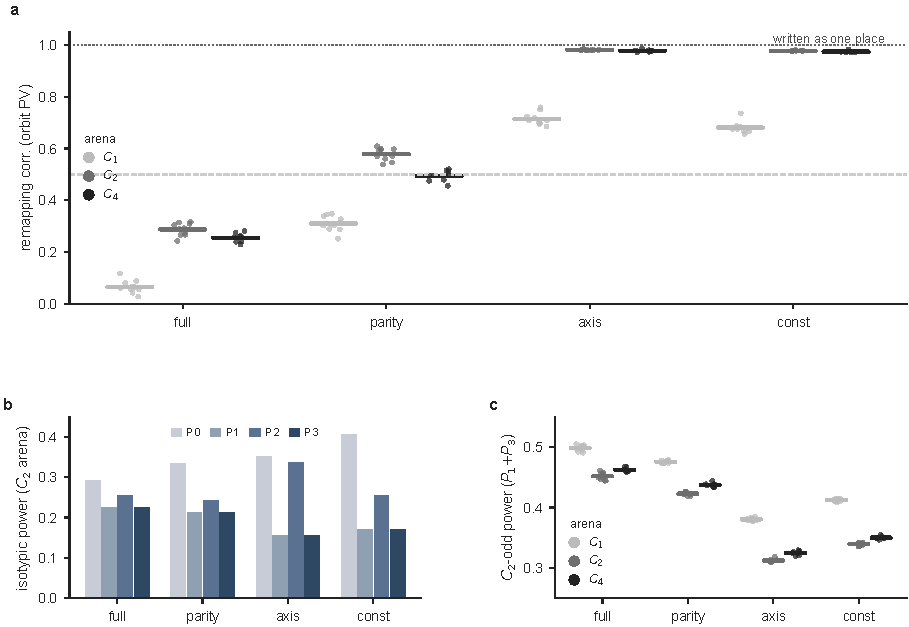
\includegraphics[width=\textwidth]{figures/fig_population.pdf}
\caption{\textbf{The quotient in the population code.} (\textbf{a}) Remapping, read as the
population-vector correlation between a position and its symmetry image  (Leutgeb et al., 2005) (one dot
per network; bar, mean). Under the invariant encodings (\textit{axis}, \textit{const}) the
correlation reaches $\approx0.98$ in the $C_2$ and $C_4$ arenas, the two copies are written as one
place, while \textit{full} separates them ($\approx0.28$) and the matched \textit{parity} is
intermediate ($0.58$ in $C_2$). (\textbf{b}) Isotypic power spectrum ($C_2$ arena): the invariant
encodings concentrate power in the even characters ($P_0$, $P_2$) and suppress the odd ones
($P_1$, $P_3$), the representation-theoretic content the encoding's invariance dictates.
(\textbf{c}) $C_2$-odd power $P_1{+}P_3$ by encoding and arena: lower for the invariant encodings
and falling into the symmetric arenas, the descriptive correlate of the fold. Arenas
$C_1$/$C_2$/$C_4$.}
\label{figS:population}
\end{figure}

\end{document}
